\documentclass[10pt,landscape,a4paper]{article}
%\usepackage[utf8]{inputenc}
%\usepackage[ngerman]{babel}
\usepackage[normalem]{ulem}
\usepackage{tikz}
\usetikzlibrary{shapes,positioning,arrows,fit,calc,graphs,graphs.standard}
\usepackage[nosf]{kpfonts}
\usepackage[t1]{sourcesanspro}
%\usepackage[lf]{MyriadPro}
%\usepackage[lf,minionint]{MinionPro}
\usepackage{multicol}
\usepackage{wrapfig}
\usepackage[top=0mm,bottom=1mm,left=0mm,right=1mm]{geometry}
\usepackage[framemethod=tikz]{mdframed}
\usepackage{microtype}
%\usepackage{physics}
\usepackage{tabularx}
\usepackage{hhline}
\usepackage{makecell}
\usepackage{mathtools}
\usepackage{amssymb}
% add to preamble
\usepackage{booktabs}

% allow captions outside float environments (useful inside multicols)
\usepackage{caption}

\usepackage{listings}

\DeclarePairedDelimiter{\ceil}{\lceil}{\rceil}

\newcommand\codeblue[1]{\textcolor{blue}{\code{#1}}}

\usepackage{lastpage}
\usepackage{datetime}
\yyyymmdddate
\renewcommand{\dateseparator}{-}
\let\bar\overline

\definecolor{myblue}{cmyk}{1,.72,0,.38}

\def\firstcircle{(0,0) circle (1.5cm)}
\def\secondcircle{(0:2cm) circle (1.5cm)}

\colorlet{circle edge}{myblue}
\colorlet{circle area}{myblue!5}

\tikzset{filled/.style={fill=circle area, draw=circle edge, thick},
outline/.style={draw=circle edge, thick}}

\pgfdeclarelayer{background}
\pgfsetlayers{background,main}

%\everymath\expandafter{\the\everymath \color{myblue}}
%\everydisplay\expandafter{\the\everydisplay \color{myblue}}


\renewcommand{\baselinestretch}{.8}
\pagestyle{empty}

\global\mdfdefinestyle{header}{%
  linecolor=gray,linewidth=1pt,%
  leftmargin=0mm,rightmargin=0mm,skipbelow=0mm,skipabove=0mm,
}

\newcommand{\header}{
  \begin{mdframed}[style=header]
    \footnotesize
    \sffamily
    HSI1000 Finals Cheatsheet v1.1 (\today)\\
    by~Dumboiroy,~page~\thepage~of~\pageref{LastPage}
  \end{mdframed}
}

\let\counterwithout\relax
\let\counterwithin\relax
\usepackage{chngcntr}

\usepackage{verbatim}

\usepackage{etoolbox}
\makeatletter
\preto{\@verbatim}{\topsep=0pt \partopsep=0pt }
\makeatother

\counterwithin*{equation}{section}
\counterwithin*{equation}{subsection}
\usepackage{enumitem}
\newlist{legal}{enumerate}{10}
\setlist[legal]{label*=\arabic*.,leftmargin=2.5mm}
\setlist[itemize]{leftmargin=3mm}
\setlist[enumerate]{leftmargin=3.5mm}
\setlist{nosep}
\usepackage{minted}

\def\code#1{\texttt{#1}}

\newenvironment{descitemize} % a mixture of description and itemize
{\begin{description}[leftmargin=*,before=\let\makelabel\descitemlabel]}
{\end{description}}

\newcommand{\descitemlabel}[1]{%
  \textbullet\ \textbf{#1}%
}
\makeatletter



\renewcommand{\section}{\@startsection{section}{1}{0mm}%
  {.2ex}%
  {.2ex}%x
{\color{myblue}\sffamily\small\bfseries}}
\renewcommand{\subsection}{\@startsection{subsection}{1}{0mm}%
  {.2ex}%
  {.2ex}%x
{\sffamily\bfseries}}
\renewcommand{\subsubsection}{\@startsection{subsubsection}{1}{0mm}%
  {.2ex}%
  {.2ex}%x
{\rmfamily\bfseries}}

\global\let\tikz@ensure@dollar@catcode=\relax

\def\mathcolor#1#{\@mathcolor{#1}}
\def\@mathcolor#1#2#3{%
  \protect\leavevmode
  \begingroup
  \color#1{#2}#3%
  \endgroup
}

\makeatother
\setlength{\parindent}{0pt}

\setminted{tabsize=2, breaklines}
% Remove belowskip of minted
\setlength\partopsep{-\topsep}

\newcolumntype{a}{>{\hsize=1.5\hsize}X}
% \newcolumntype{b}{>{\hsize=.25\hsize}X}

\setlength\columnsep{1.5pt}
\setlength\columnseprule{0.1pt}

\begin{document}
\setlength{\abovedisplayskip}{0pt}
\setlength{\belowdisplayskip}{0pt}

\header

\scriptsize
\begin{multicols*}{4}
  \raggedcolumns
  \section{Confidence Interval Calculation}
  % Use a non-floating, captioned table so it appears inside multicols
  \begin{center}
    {
      \captionsetup{font=footnotesize}
      \captionof{table}{Table 5.1 for Approx. Margin of Error (\%)}
    }
    \begin{tabular}{lr}
      \toprule
      Sample Size & Approx. Margin of Error (\%)\textsuperscript{*} \\
      \midrule
      25          & $\pm 22$                                        \\
      50          & $\pm 14$                                        \\
      100         & $\pm 10$                                        \\
      250         & $\pm 6$                                         \\
      500         & $\pm 4$                                         \\
      1000        & $\pm 3$                                         \\
      1500        & $\pm 2.5$                                       \\
      2000        & $\pm 2$                                         \\
      \bottomrule
    \end{tabular}

    \vspace{4pt}
    \footnotesize\textit{\textsuperscript{*}The interval surrounding the actual sample outcome containing 95\% of all possible sample outcomes.}
  \end{center}

  \subsection{Proportion of values (e.g. conf interval for correct predictions)}
  \begin{enumerate}
    \item Sample Proportion: $\hat{p} = \frac{n_{\text{True}}}{n}$
    \item Standard Error: $SE = \sqrt{\frac{\hat{p}(1 - \hat{p})}{n}}$
    \item Confidence Interval: $\text{CI} = \hat{p} \pm z \cdot SE$
  \end{enumerate}
  \subsection{Confidence interval of mean}
  \begin{enumerate}
    \item Sample Mean: $\bar{x} = \frac{1}{n}\sum_{i=1}^{n} x_i$
    \item Standard Error: $SE = \frac{s}{\sqrt{n}}$
    \item Confidence Interval: $\text{CI} = \bar{x} \pm z \cdot SE$
  \end{enumerate}  \subsection{CI Overlap Rules of Thumb (Heuristic)}
  \subsubsection{Conditions}
  \begin{itemize}
    \item One of the CI must be \textbf{control group}.
    \item Both groups must be \textbf{independent} (RCT or equivalent, no pairing).
    \item Same variable, same conditions
  \end{itemize}
  \subsubsection{Rules of thumb:}
  Let two $95\%$ confidence intervals be $[L_1, U_1]$ and $[L_2, U_2]$. Overlap = Overlap in CIs.
  \begin{enumerate}
    \item No overlap -> difference is statistically significant at the $95\%$ confidence level.
    \item Overlap $< \frac{1}{3} \times$ range covered by the CIs -> could be statistically significant. Bigger Overlap -> less confidence.
    \item Overlap $> \frac{1}{3} \times$ range covered by the CIs -> difference is probably not statistically significant.
  \end{enumerate}
  \textit{Note: This is a heuristic approximation, to be used because HSI taught this.}

  \section{Lecture 1: The Founding of Modern Science}
  \begin{itemize}
    \item Science emerged as a formal method during the Scientific Revolution (1543 De Revolutionibus → 1687 Principia).
    \item Key figures (Copernicus, Galileo, Kepler, Bacon, Newton) shifted from Aristotelian views to evidence-based understanding.
    \item The steam engine and Industrial Revolution show how discoveries enabled technological and societal transformation.
  \end{itemize}

  \section{Lecture 2: The Baloney Toolkit Applied to a Simple Investigation}
  \begin{enumerate}[label=\arabic*.]
    \item Source reliability: credentials · lateral reading
    \item Perspective: funding/purpose → bias
    \item Positive evidence: supports · reliable · relevant · accurate data
    \item Evidence consensus: majority viewpoint
    \item Verified independently: reproduction · peer-review · fact-check
    \item Sound reasoning: no fallacies · correct logic
  \end{enumerate}

  \textit{Prep:} skeptical mindset · aware of own biases · guard emotions


  \section{Lecture 3: Scientific Explanations and Models}
  \begin{itemize}
    \item Explanations must account for observations and be falsifiable (capable of being proven wrong).
    \item Models are simplified representations that help understand complex systems.
    \item Understand models' limitations and assumptions before applying them to real situations.
  \end{itemize}

  \section{Lecture 4: Experimentation and Uncertainty}
  \begin{itemize}
    \item All measurements have inherent uncertainty; precision indicates reliable significant figures.
    \item Accuracy compares the mean to the true value; uncertainty in averages is expressed as margin of error (commonly 95% CI).
    \item Validate and calibrate instruments/methods to remove systematic errors and ensure true measurements.
  \end{itemize}

  \section{Lecture 5: The Science of Climate Change}
  \subsection{Climate Change Myths and Truths}

  \begin{enumerate}
    \item \textbf{Myth: Climate's Changed Before}
          \begin{itemize}
            \item[$\times$] Natural cycles $\to$ current warming natural
            \item[$\checkmark$] Milankovitch cycles, solar radiation: exist
            \item[$\checkmark$] Current warming: unprecedented (rate \& magnitude, 170 yrs)
            \item[$\checkmark$] Driver: human GHG $\not\equiv$ natural variation
          \end{itemize}

    \item \textbf{Myth: It's the Sun}
          \begin{itemize}
            \item[$\times$] Solar activity $\to$ warming
            \item[$\checkmark$] Past 40 yrs: solar $\downarrow$ slight, temps $\uparrow$ significant
            \item[$\checkmark$] Pattern (strat cool, tropics warm): GHG forcing $\not\equiv$ solar
            \item[$\checkmark$] Sun: not primary driver
          \end{itemize}

    \item \textbf{Myth: Animals \& Plants Adapt}
          \begin{itemize}
            \item[$\times$] Flora/fauna $\to$ adapt
            \item[$\checkmark$] Extinction: 100--1000$\times$ baseline
            \item[$\checkmark$] Pace too rapid: no adaptation time
            \item[$\checkmark$] Outcome: species extinction
          \end{itemize}

    \item \textbf{Myth: Earth Cooling}
          \begin{itemize}
            \item[$\times$] Warming stopped, cooling now
            \item[$\checkmark$] Cherry-picking time windows: false
            \item[$\checkmark$] Full dataset: $\uparrow$ unambiguous
            \item[$\checkmark$] 2010s: warmest decade
          \end{itemize}

    \item \textbf{Myth: It's Not Us}
          \begin{itemize}
            \item[$\times$] Climate change $\not\Rightarrow$ human
            \item[$\checkmark$] 10 fingerprints:
                  \begin{enumerate}
                    \item CO$_2$: 30 Gt/yr $\uparrow$
                    \item O$_2$: $\downarrow$
                    \item Fossil fuel carbon signature
                    \item Coral carbon absorption
                    \item Heat escape: specific wavelengths
                    \item Atmosphere: shrinking
                    \item Nights: warming faster
                    \item Troposphere: warm, stratosphere: cool
                    \item Ocean heat: $\uparrow$
                    \item Fossil carbon: $\uparrow$ in air
                  \end{enumerate}
          \end{itemize}
  \end{enumerate}

  \textbf{Global Warming Evidence}
  \begin{itemize}
    \item All indicators $\uparrow$ (as expected GHG):
          \begin{itemize}
            \item Land surface temps
            \item Sea surface temps
            \item Ocean heat (90\% of total)
            \item Sea level
            \item Glacier melt (Arctic ice $\downarrow$ 35\% since '79)
            \item Snow cover $\downarrow$
            \item Humidity $\uparrow$
          \end{itemize}
  \end{itemize}

  \textbf{Five Denial Forms}
  \begin{enumerate}
    \item Science: ``no consensus''
    \item Economic: ``too costly''
    \item Humanitarian: ``net benefit''
    \item Political: ``others act first''
    \item Crisis: ``uncertainty $\to$ inaction''
  \end{enumerate}

  \textbf{Cognitive Biases}
  \begin{itemize}
    \item Time-discount: future $\downarrow$ valued
    \item Optimism: ``tech solves it''
    \item Control illusion: ``scientists fix''
    \item Egocentrism: ``others blame''
  \end{itemize}
  \section*{Atmospheric Mechanisms of Climate Change}

  \subsection*{Atmospheric Composition \& Greenhouse Gases}
  \begin{itemize}
    \item Major gases: $N_2$ (78\%), $O_2$ (21\%), Ar (1\%)
    \item Trace gases (greenhouse effect):
          \begin{itemize}
            \item $CO_2$: $\sim$420 ppm (pre-industrial: 280 ppm)
            \item $CH_4$: $\sim$1900 ppb
            \item $N_2O$: $\sim$335 ppb
          \end{itemize}
    \item Greenhouse gases $\rightarrow$ absorb infrared radiation $\rightarrow$ trap heat
  \end{itemize}

  \subsection*{Infrared Radiation \& Energy Balance}
  \begin{itemize}
    \item Solar constant: $S = 1370$ W m$^{-2}$
    \item Earth cross-section: $\pi R^2$ $\rightarrow$ absorbed energy: $S \times \pi R^2 / 4 \pi R^2 = S/4$
    \item Stefan-Boltzmann law: $P = \sigma T^4$ (emitted energy $\propto T^4$)
    \item IR wavelengths: 12--18 $\mu$m (thermal radiation from Earth)
    \item $CO_2$ absorption: 90$\times$ more effective than air
    \item $H_2O$ absorption: 16,000$\times$ more effective than air
    \item Atmosphere: transparent to incoming solar radiation $\leftrightarrow$ opaque to outgoing IR
  \end{itemize}

  \subsection*{Temperature \& Greenhouse Effect}
  \begin{itemize}
    \item Without atmosphere: $T_E \approx -18$ $^\circ$C (calculated from energy balance)
    \item With atmosphere (greenhouse effect): $T_E \approx +15$ $^\circ$C (observed)
    \item Difference: $\sim 33$ $^\circ$C warming due to greenhouse gases
    \item Mechanism:
          \begin{enumerate}
            \item Atmosphere absorbs outgoing IR radiation
            \item Atmosphere re-emits radiation in all directions (including back to surface)
            \item Additional downward radiation $\rightarrow$ surface warming
          \end{enumerate}
    \item $CO_2$ increase $\rightarrow$ more IR absorption $\rightarrow$ higher surface temperature
  \end{itemize}

  \subsection*{Carbon Dioxide \& Causal Chains}
  \begin{itemize}
    \item Fossil fuel combustion $\rightarrow$ $CO_2$ emissions $\rightarrow$ atmospheric $CO_2$ $\uparrow$
    \item Rising $CO_2$ (280 $\rightarrow$ 420 ppm since 1750):
          \begin{itemize}
            \item Due to: coal, oil, natural gas burning
            \item Confirmed by: carbon-14 isotope ratios (fossil fuels lack $^{14}$C)
          \end{itemize}
    \item $CO_2$ increase $\rightarrow$ IR absorption $\uparrow$ $\rightarrow$ temperature $\uparrow$
    \item Temperature rise unprecedented in past 800,000 years (ice core records)
  \end{itemize}

  \subsection*{Troposphere \& Stratosphere}
  \begin{itemize}
    \item \textbf{Troposphere} (lower atmosphere):
          \begin{itemize}
            \item Height: 0--12 km (varies: $\sim$8 km poles, $\sim$18 km equator)
            \item Temperature: decreases with altitude ($\sim$6.5 $^\circ$C per km)
            \item Contains: weather systems, clouds, 80\% of atmosphere's mass
            \item Greenhouse effect warming occurs here
          \end{itemize}
    \item \textbf{Stratosphere} (upper atmosphere):
          \begin{itemize}
            \item Height: 12--50 km
            \item Temperature: increases with altitude (inversion due to ozone)
            \item Contains: ozone layer ($\sim$20--25 km altitude)
          \end{itemize}
    \item Boundary (tropopause): temperature minimum ($\sim$-57 $^\circ$C)
  \end{itemize}

  \subsection*{UV Radiation \& Stratospheric Processes}
  \begin{itemize}
    \item Solar UV radiation $\rightarrow$ reaches upper atmosphere
    \item Ozone formation: $O_2$ (UV) $\rightarrow$ O $\rightarrow$ $O_3$ (ozone)
    \item Ozone role: absorbs UV radiation $\rightarrow$ protects surface $\rightarrow$ heats stratosphere
    \item Temperature structure:
          \begin{itemize}
            \item Troposphere (cools with altitude): due to greenhouse effect dominance
            \item Stratosphere (warms with altitude): due to UV + ozone heating
          \end{itemize}
    \item CFCs $\rightarrow$ ozone depletion $\rightarrow$ less UV absorption $\rightarrow$ more surface UV
  \end{itemize}

  \subsection*{What Affects What: Causal Mechanisms}
  \begin{center}
    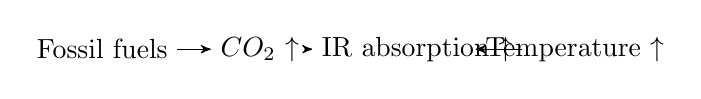
\begin{tikzpicture}[node distance=2cm, auto, >=stealth']
      \node (fossil) {Fossil fuels};
      \node (co2) [right of=fossil] {$CO_2$ $\uparrow$};
      \node (ir) [right of=co2] {IR absorption $\uparrow$};
      \node (temp) [right of=ir] {Temperature $\uparrow$};

      \path [->] (fossil) edge (co2)
      (co2) edge (ir)
      (ir) edge (temp);
    \end{tikzpicture}
  \end{center}

  \begin{itemize}
    \item Solar input ($\sim$1370 W/$m^2$) $\rightarrow$ relatively constant
    \item $CO_2$ concentration $\rightarrow$ controls fraction of IR trapped
    \item Atmospheric composition $\rightarrow$ determines temperature equilibrium
    \item Temperature $\rightarrow$ drives all climate effects (precipitation, sea level, ecosystems)
  \end{itemize}

  \subsection*{Energy Balance Model (Summary)}
  \begin{itemize}
    \item Energy in: Solar radiation absorbed $= S \times (1-A) \times \pi R^2 / 4$
          \begin{itemize}
            \item $S$: solar constant
            \item $A$: albedo (reflectivity $\sim 0.3$)
          \end{itemize}
    \item Energy out: IR radiation emitted $= \sigma T_E^4 \times 4\pi R^2$
    \item Equilibrium: Energy in $=$ Energy out $\rightarrow$ Solve for $T_E$
    \item Greenhouse effect: reduce effective emissivity $\rightarrow$ higher $T_E$ at equilibrium
    \item More $CO_2$ $\rightarrow$ lower effective emissivity $\rightarrow$ higher $T_E$
  \end{itemize}



  \section{Lecture 6: Modelling Climate Change}

  % \begin{tabular}{l}
  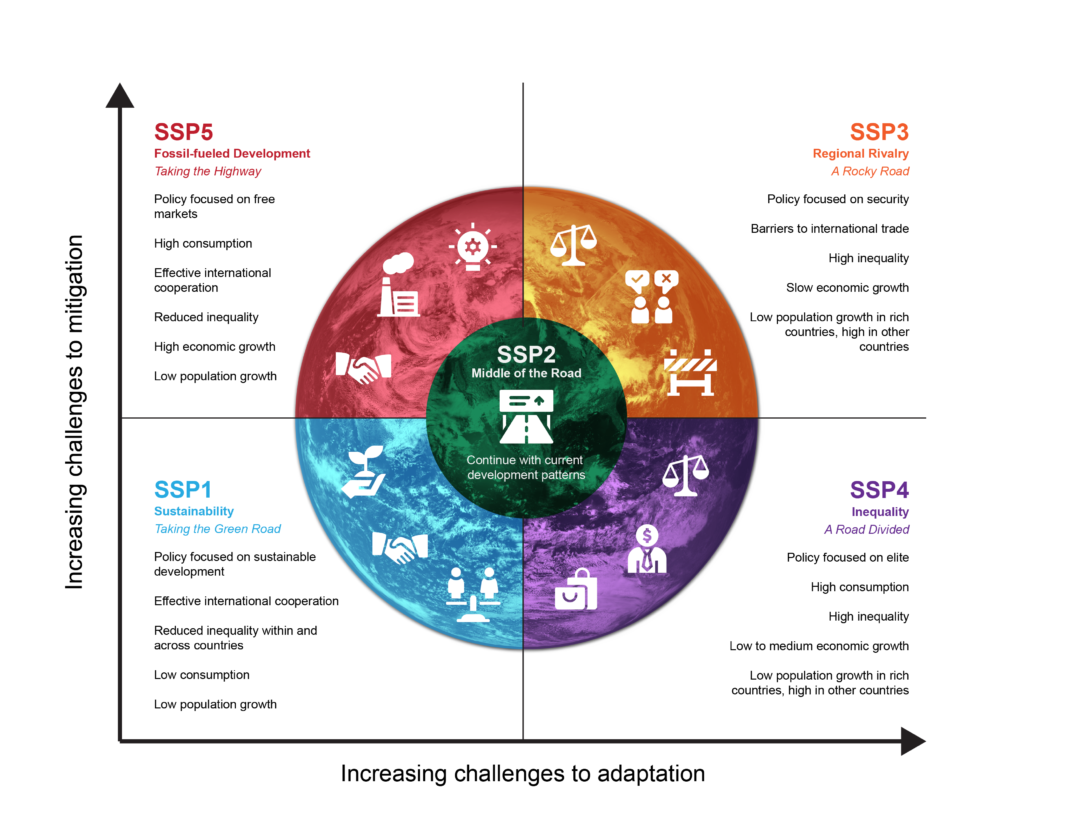
\includegraphics[width=1\linewidth]{ssp-matrix}
  % \end{tabular}
  % \begin{minipage}{0.15\columnwidth}
  %   Placeholder note for image
  % \end{minipage}


  \subsection*{SSP 1: Scientific Consensus History}
  \begin{itemize}
    \item Describe establishment of scientific consensus on climate change
    \item Include role of IPCC: Intergovernmental Panel on Climate Change
    \item Track: 1979 First Assessment $\to$ 1995 Second Assessment (discernible impact) $\to$ 2001 Third Assessment (mostly due to humans)
  \end{itemize}

  \subsection*{SSP 2: Climate vs Weather \& Greenhouse Effect vs Climate Change}
  \begin{itemize}
    \item \textbf{Climate}: average weather over long period in a region
    \item \textbf{Weather}: short-term atmospheric conditions $\to$ temporal scale: days
    \item \textbf{Greenhouse effect}: GHGs trap IR radiation $\to$ warming (natural process)
    \item \textbf{Climate change}: shift in average climate conditions $\to$ temporal scale: decades/centuries
    \item Distinction: global warming (cause) $\Rightarrow$ climate change (effect)
  \end{itemize}

  \subsection*{SSP 3: Proxy Methods for Past Temperature Reconstruction}
  \begin{itemize}
    \item \textbf{Dendroclimatology}: tree ring width $\propto$ growth conditions $\Rightarrow$ historical climate estimate
    \item \textbf{Coral records}: oxygen isotope ratios in carbonate shells $\propto$ temperature
    \item \textbf{Ice cores}: composition of trapped air bubbles $\Rightarrow$ atmospheric conditions; oxygen isotopes $\propto$ temperature
    \item \textbf{Paleoclimate proxies}: calibrated against modern measurements $\Rightarrow$ extend record backwards
    \item Data: 800,000 years available; recent warming unprecedented in last 2,000 years
  \end{itemize}

  \subsection*{SSP 4: Public vs Scientific Consensus Gap}
  \begin{itemize}
    \item \textbf{Scientific consensus}: 97.1\% of peer-reviewed papers agree on anthropogenic climate change
    \item \textbf{Public perception}: 1997 only 48\% believed consensus $\to$ 2021 rose to 68\% (still below actual)
    \item Disconnect: public underestimates scientist agreement on climate change reality
    \item Oreskes (2004): 928 papers surveyed, 100\% agreed; 0\% rejected consensus
  \end{itemize}

  \subsection*{SSP 5: Establishment of Scientific Consensus}
  \begin{itemize}
    \item \textbf{Evidence requirements}: (1) observational data showing warming, (2) temperature rise unusual, (3) GHG increases, (4) CO$_2$ rise from fossil fuels
    \item \textbf{Key evidence}:
          \begin{enumerate}
            \item Instrumental record: NASA, NOAA, Met Office all show $\sim$1.1°C rise since pre-industrial
            \item Proxy records: trees, coral, ice cores $\Rightarrow$ current warming unprecedented in 800,000 years
            \item CO$_2$ rise: 315 ppm (1958) $\to$ 415+ ppm (today); Keeling curve shows continuous increase
            \item Carbon-14 effect (Suess): fossil fuels dilute atmospheric $^{14}$C $\Rightarrow$ directly proves fossil fuel origin
          \end{enumerate}
    \item \textbf{Verification}: multiple independent datasets, methods, organizations all converge $\Rightarrow$ consensus achieved
    \item \textbf{Consensus definition}: majority of scientists agree based on verified evidence, not authority
  \end{itemize}

  \section{Lecture 7: On the Mongering of Doubt}
  \begin{itemize}
    \item Scientific uncertainty is sometimes misrepresented as disagreement to cast doubt on established findings.
    \item Well-funded campaigns manufacture doubt using tactics similar to those of the tobacco industry.
    \item Media and political polarization amplify manufactured doubt despite overwhelming evidence.
  \end{itemize}

  \section{Lecture 8: The Reliability of Climate Change Predictions}
  \begin{itemize}
    \item Climate predictions compare well with observed data and have proven reliable in many cases.
    \item Individual models vary; ensemble and trend analyses show consistency with observations.
    \item Confidence arises from multiple independent lines of evidence converging on similar conclusions.
  \end{itemize}

  \section{Lecture 9: Restoration of Nature (Sample Science)}
  \begin{itemize}
    \item Restoration ecology applies scientific methods to return degraded ecosystems to functional, biodiverse states.
    \item Understanding ecological processes and species interactions is essential for successful restoration.
    \item Long-term monitoring and adaptive management allow strategy adjustments based on outcomes.
  \end{itemize}

  \section{Lecture 10: Connectivity of Nature (Sample Science)}
  \begin{itemize}
    \item Ecological connectivity—movement between habitat patches—is critical for biodiversity conservation.
    \item Fragmentation reduces connectivity, isolating populations and lowering genetic diversity and resilience.
    \item Corridors and connected protected-area networks enable movement and maintain ecosystem function.
  \end{itemize}

  \section{Lecture 11: Hinterland of Resources (Sample Science)}
  \begin{itemize}
    \item Resource hinterlands that supply cities often suffer significant environmental degradation.
    \item Understanding resource flows and ecological costs is key for sustainable management.
    \item Local and regional policies shape extraction practices and environmental impacts.
  \end{itemize}

  \section{Lecture 12: Fallacies in the Name of Science \& Course Wrap Up}
  \begin{itemize}
    \item Common logical fallacies (appeal to authority, straw man, ad hominem) misrepresent scientific claims.
    \item Understanding science, its limits, and proper evidence evaluation guards against pseudoscience.
    \item Science is powerful for understanding the natural world but must be applied critically, aware of uncertainty and evidence.
  \end{itemize}

  \subsection{Fallacies \& Cognitive Biases}
  \begin{itemize}
    \item \textbf{False Anomaly}: Presenting an expected or documented phenomenon as mysterious, then invoking extraordinary explanations while ignoring simpler, documented causes (e.g., crop circles blamed on aliens while ignoring tractor tramlines).
    \item \textbf{Questionable Arguments by Elimination}: Ruling out some alternatives does not prove the remaining hypothesis (eliminating luck doesn't prove ESP).
    \item \textbf{Illicit Causal Inferences (Post hoc)}: Inferring causation from correlation or temporal proximity (thinking of a friend then they call $\neq$ your thought caused the call).
    \item \textbf{Unsupported Analogies}: Using analogies or superficial similarities as evidence when they do not justify the inference (e.g., moon→tides so planets→personality).
    \item \textbf{Untestable Explanations \& Predictions}: Claims that cannot be empirically falsified are unscientific; conspiracy theories often evade falsification by treating absence of evidence as "proof" of a cover-up.
    \item \textbf{Empty Jargon}: Stringing together scientific-sounding but meaningless terms to create an appearance of expertise (e.g., "quantum entanglement telekinesis").
    \item \textbf{Ad Hoc Rescues}: Continuously modifying a claim to accommodate contrary evidence instead of revising or abandoning the claim.
    \item \textbf{Exploiting Uncertainty}: Weaponizing legitimate scientific uncertainty about details to cast doubt on well-established conclusions (e.g., using model uncertainty to deny consensus on climate change).
    \item \textbf{Confirmation Bias / Cherry-picking}: Selecting evidence that supports a preferred view while ignoring contradictory data.
    \item \textbf{Appeal to Authority / False Authority}: Accepting a claim solely because an alleged authority says so, especially when outside their expertise.
    \item \textbf{Straw Man}: Misrepresenting an opponent's argument to make it easier to attack.
    \item \textbf{Anecdotal Evidence}: Treating isolated stories or anecdotes as proof against systematic data.
    \item \textbf{False Equivalence}: Presenting two unequal arguments or bodies of evidence as if they were equivalent.
  \end{itemize}

  \subsection{Cognitive Profile: Dunning--Kruger Effect}
  \begin{itemize}
    \item Low-ability individuals tend to overestimate their competence; conversely, highly competent people may underestimate theirs.
    \item Awareness of this effect helps interpret confident claims from non-experts and cultivates intellectual humility.
  \end{itemize}

  \subsection{Good Practices \& Non-fallacies}
  \begin{itemize}
    \item \textbf{Healthy skepticism}: Question claims constructively and demand appropriate evidence before accepting extraordinary conclusions.
    \item \textbf{Burden of proof}: Assign stronger evidential requirements to more extraordinary claims; require reproducible, falsifiable, and preferably independent evidence.
    \item Consider alternative hypotheses, actively seek disconfirming evidence, and weigh converging independent lines of evidence.
  \end{itemize}


\end{multicols*}
\end{document}
